\begin{task}[credit=4]{\codesym~Entscheidungsbäume - Klassifikation}
\label{t:dt_classification}
Im Institut Institut für Produktionstechnik und Umformmaschinen, kurz PtU\footnote{\url{https://www.ptu.tu-darmstadt.de/}}, der TU Darmstadt gibt es die Aufgabe eines Scherschneideverfahrens. Dabei wird mit Hilfe eines Stempels ein Loch in einen metallischen Werkstoff gestanzt, siehe Abbildung~\ref{fig:shearcutting}. Es gibt zwei Werkstoffe im Versuch: \texttt{CuSn6} und \texttt{16MnCr5}. Die Dicke des Materials beträgt entweder $0.4$\,mm oder $0.5$\,mm. Die Geschwindigkeit des Stempels liegt in den drei Stufen $100$, $200$ und $300$ vor.

\begin{figure}[h!]{
  \begin{minipage}{0.45\linewidth}
  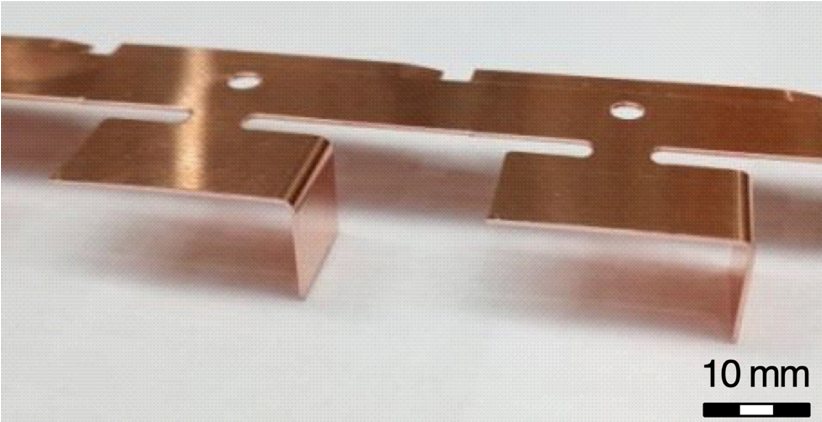
\includegraphics[width=\linewidth]{media/images/example.png}
  \end{minipage}
  \begin{minipage}{0.45\linewidth}
  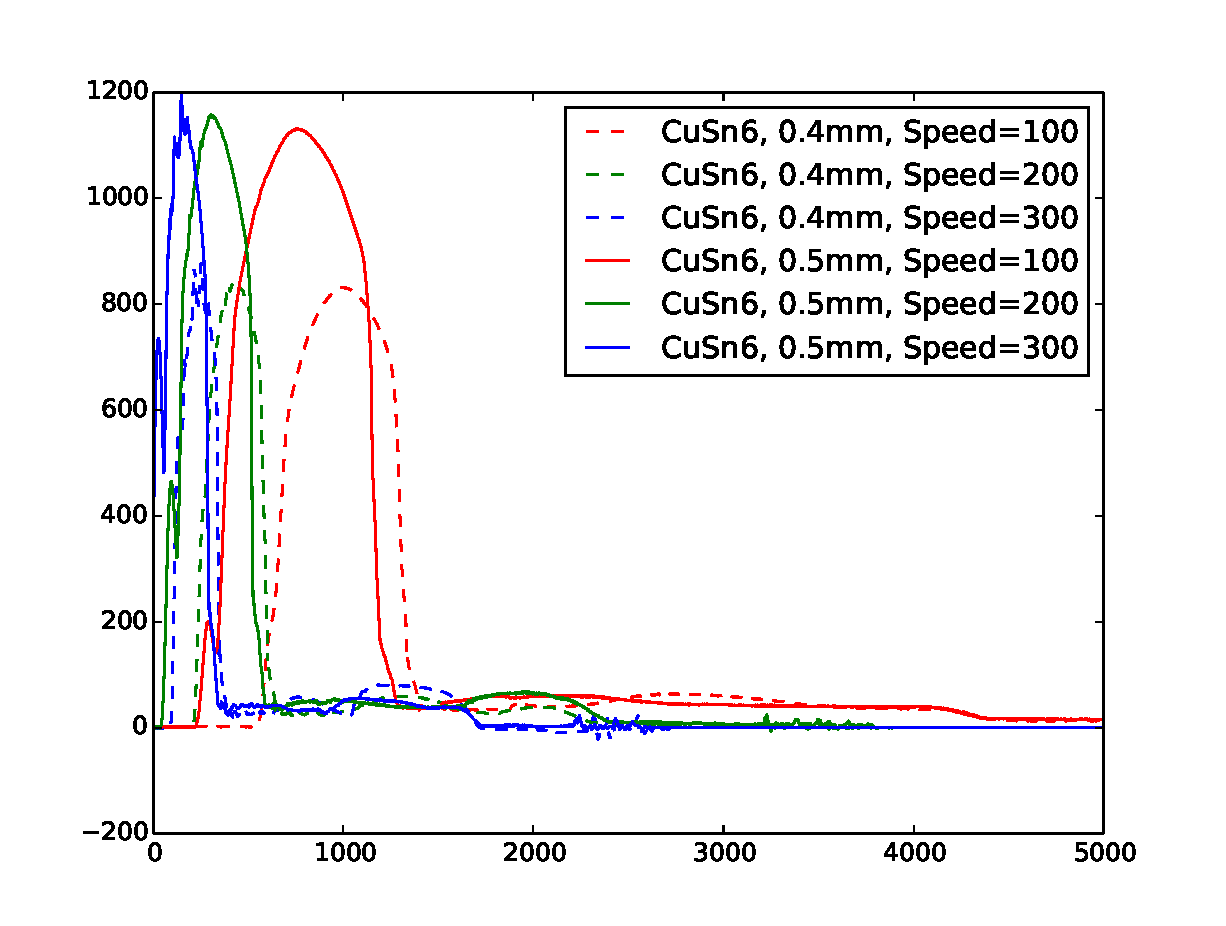
\includegraphics[width=\linewidth]{media/images/signal.pdf}%
  \end{minipage}}
  \caption{Links: Veranschaulichung des PtU Prozess. Rechts: Beispiel des Kraftsignals.}
  \label{fig:shearcutting}
 \end{figure}
 
Es gibt mehrere Sensoren, die den Status des Stanzen messen:

\begin{itemize}
 \item Kraft Sensor / Force sensor (Fz) 
 \item Verschiebungssensor / Displacement sensor (w)
 \item Beschleunigungssensor / Acceleration sensor (acc)
\end{itemize}
Im Experiment messen die Sensoren den Status des Stanzen von Beginn bis Ende jedes Prozesses.
Die Zeitreihendaten von jedem Sensor werden als 1D-Vektor dargestellt.
Das Interessante an dieser Aufgabe ist, dass der Status des Stanzen von der Art und Dicke des Materials abhängt. Andererseits ist es uns möglich, aus den Zeitreiheninformationen von den Sensoren auf die Art und Dicke des Materials und die Geschwindigkeit des Stanzen zu schließen.

\begin{itemize}
    \item \textbf{\texttt{Filename\_Fz\_raw.csv}}: Enthält Daten aus dem Kraftsensor. Jeder Zeilenvektor repräsentiert das Kraftsignal. Die Anzahl der Zeilen in der Datei beträgt $2787$, was der Anzahl der Experimente im Datensatz entspricht.
    \item \textbf{\texttt{Filename\_Speed.csv}}: Enthält die Geschwindigkeit des Schlags der $2787$ Proben.
    \item \textbf{\texttt{Filename\_thickness.csv}}: Enthält die Materialstärke der $2787$ Proben.
\end{itemize}

In dieser Übung verwenden wir die Daten des Kraftsensors, um die Proben nach der Geschwindigkeit des Stempels zu klassifizieren.

\begin{subtask}[points=3,title={\codesym~\texttt{02\_dt\_classification.py}}]
\label{t:dt_class}
Laden Sie die Daten des Kraftsensor aus \texttt{Filename\_Fz\_raw.csv} und die Geschwindigkeit des Stanzen aus \texttt{Filename\_Speed.csv} und vervollständigen Sie den Code in \texttt{02\_dt\_classification.py}:

\begin{itemize}
 \item[\codesym] Trainieren Sie einen Entscheidungsbaum zur Klassifikation in der Methode \texttt{fit\_dt\_classifier()} mithilfe von \texttt{sklearn} unter der Verwendung der Standardparameter.
 \item[\codesym] Ermitteln Sie die Testgenauigkeit in der Methode \texttt{get\_test\_accuracy()}.\\
 \item[\codesym] Plotten Sie den resultierenden Entscheidungsbaum in \texttt{export\_tree\_plot()}. Sie können dabei die Funktion \texttt{tree.export\_graphviz()} verwenden.
\end{itemize}
\end{subtask}

 \begin{subtask}[points=1,title=Visualisierung]
Zeigen Sie die erstelle Visualisierung des Entscheidungsbaumes zur Klassifikation aus Unteraufgabe~\ref{t:dt_class}.

\begin{solution}
	Es ergab sich der folgende Entscheidungsbaum:
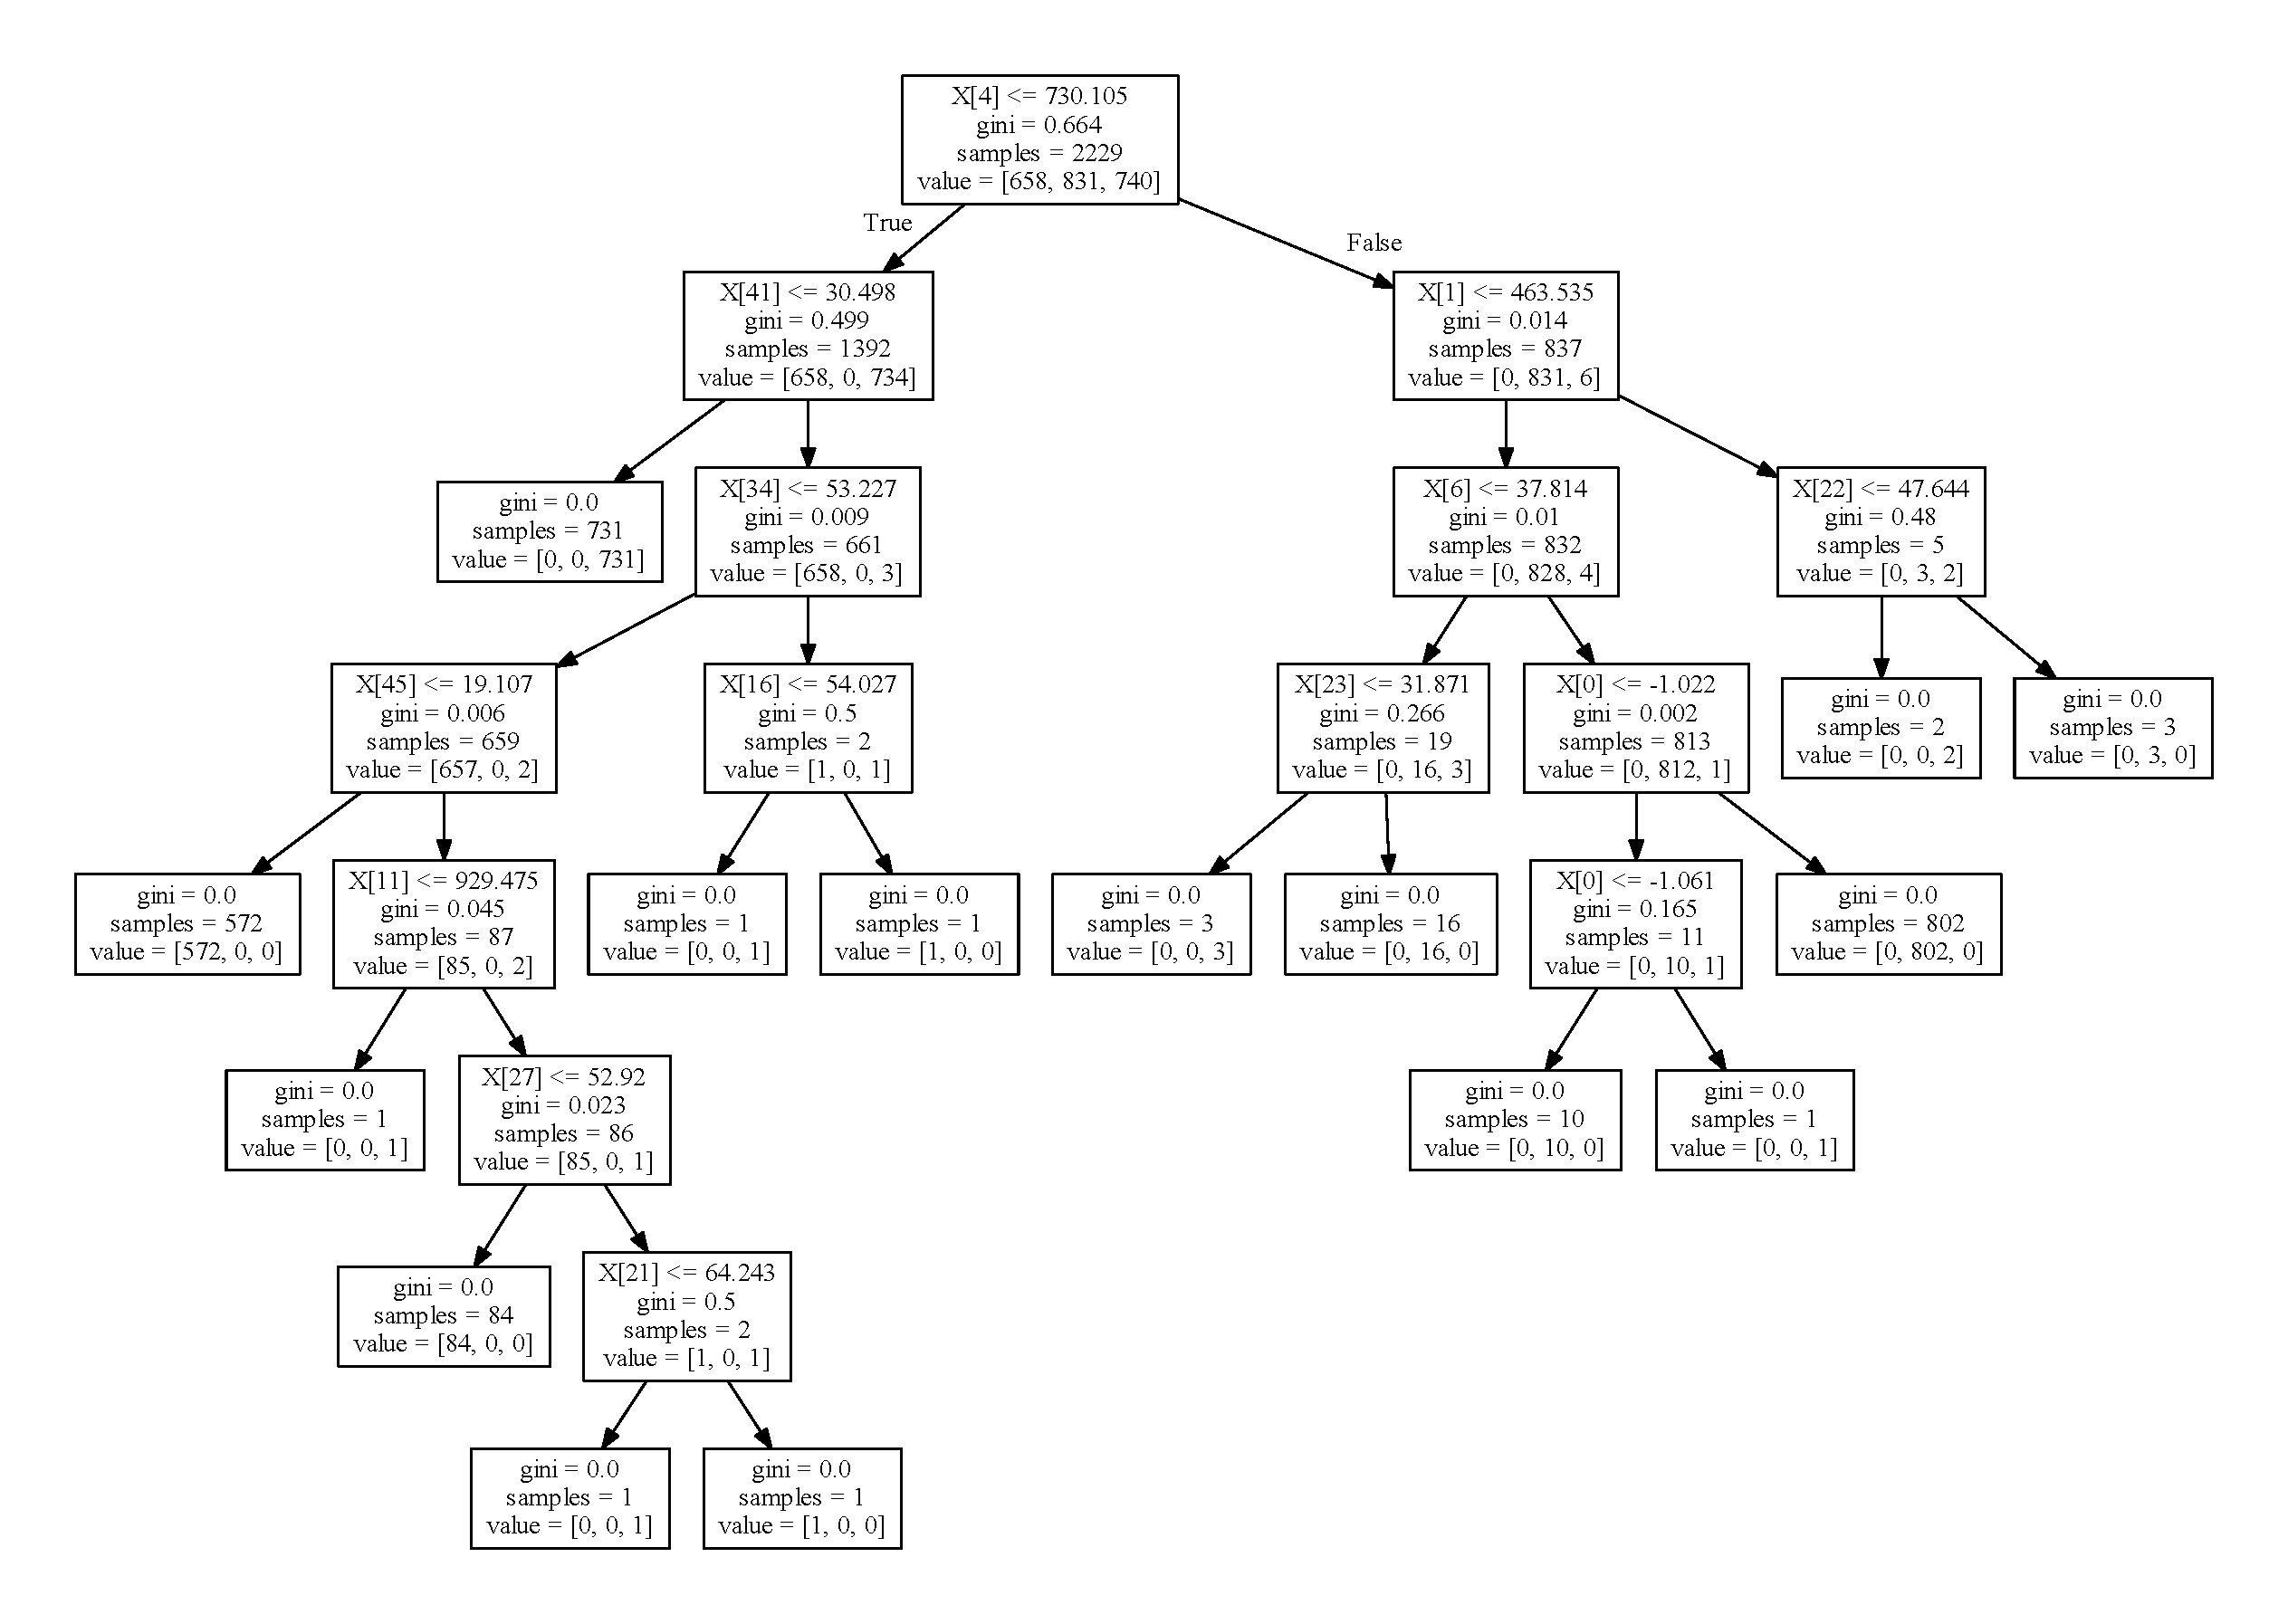
\includegraphics[width=\linewidth]{classification_tree.pdf}
\end{solution}

\end{subtask}
\end{task}

